\section{Conception}
  \begin{frame}
    \frametitle{Composants}
    \begin{figure}
    \center
		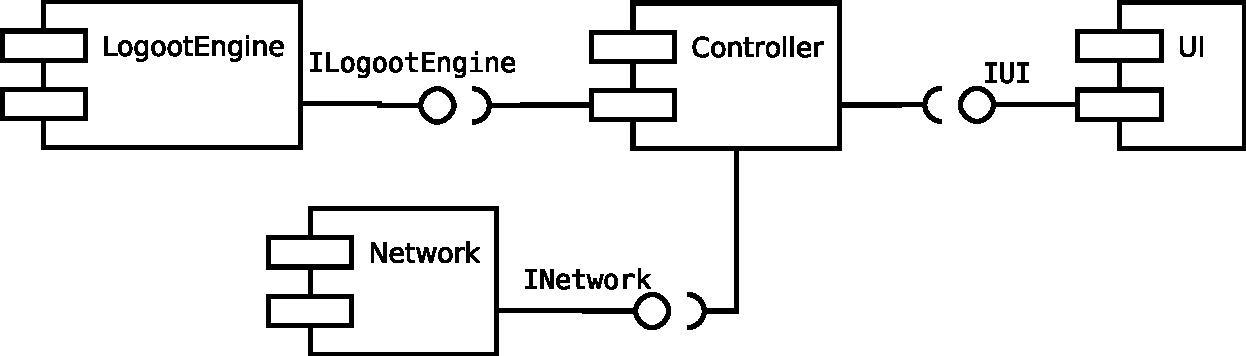
\includegraphics[scale=.5]{includes/model/architecture.pdf}
    \end{figure}
  \end{frame}

  \begin{frame}
    \frametitle{LogootEngine}
    \begin{figure}
    \center
		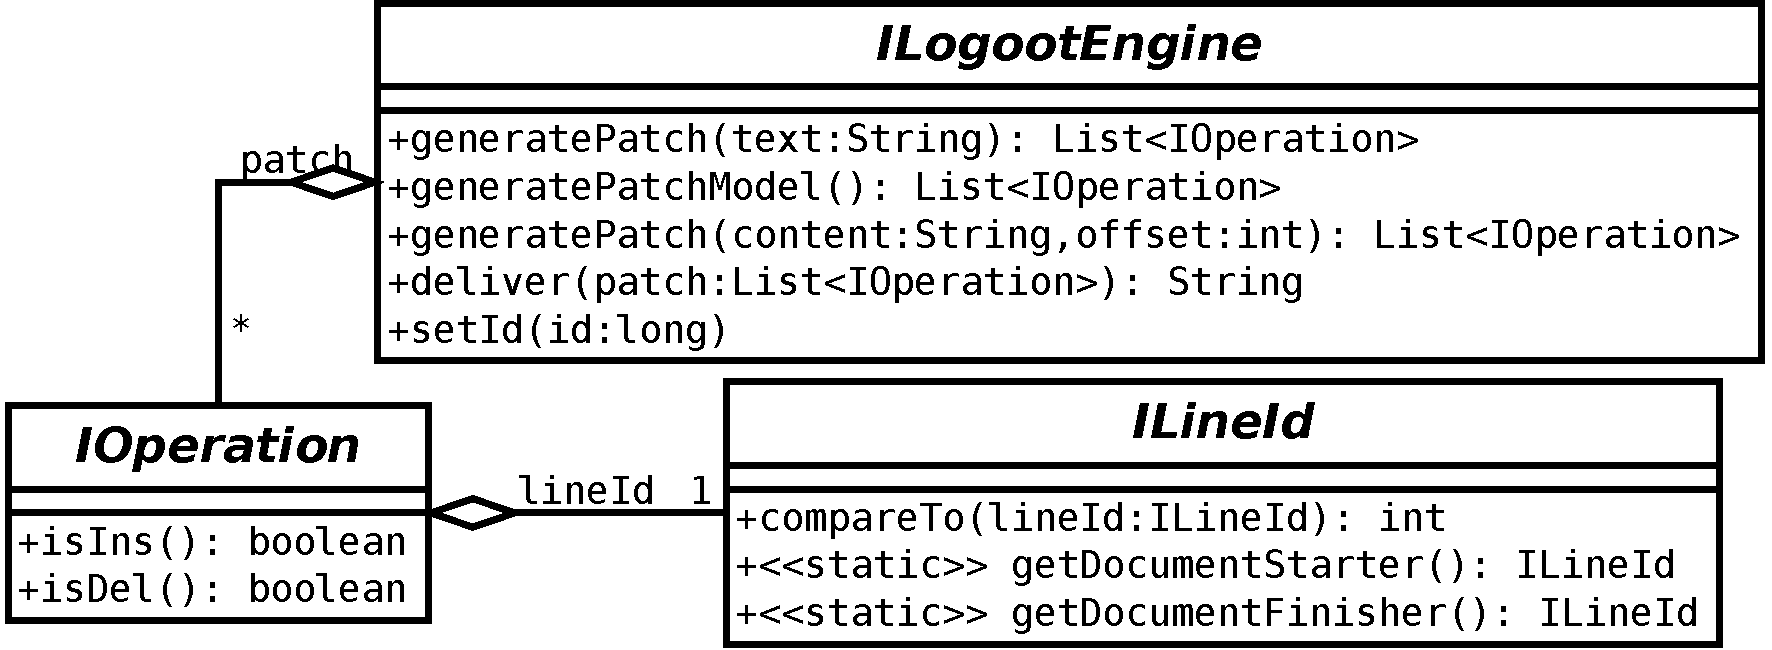
\includegraphics[scale=.3]{includes/model/ILogootEngine.pdf}
    \end{figure}
    \begin{itemize}
      \item Génération d'identifiant de ligne.
      \item Génération et Intégration de Patch.
    \end{itemize}
  \end{frame}

  \begin{frame}
    \frametitle{Network}
    \begin{figure}
    \center
		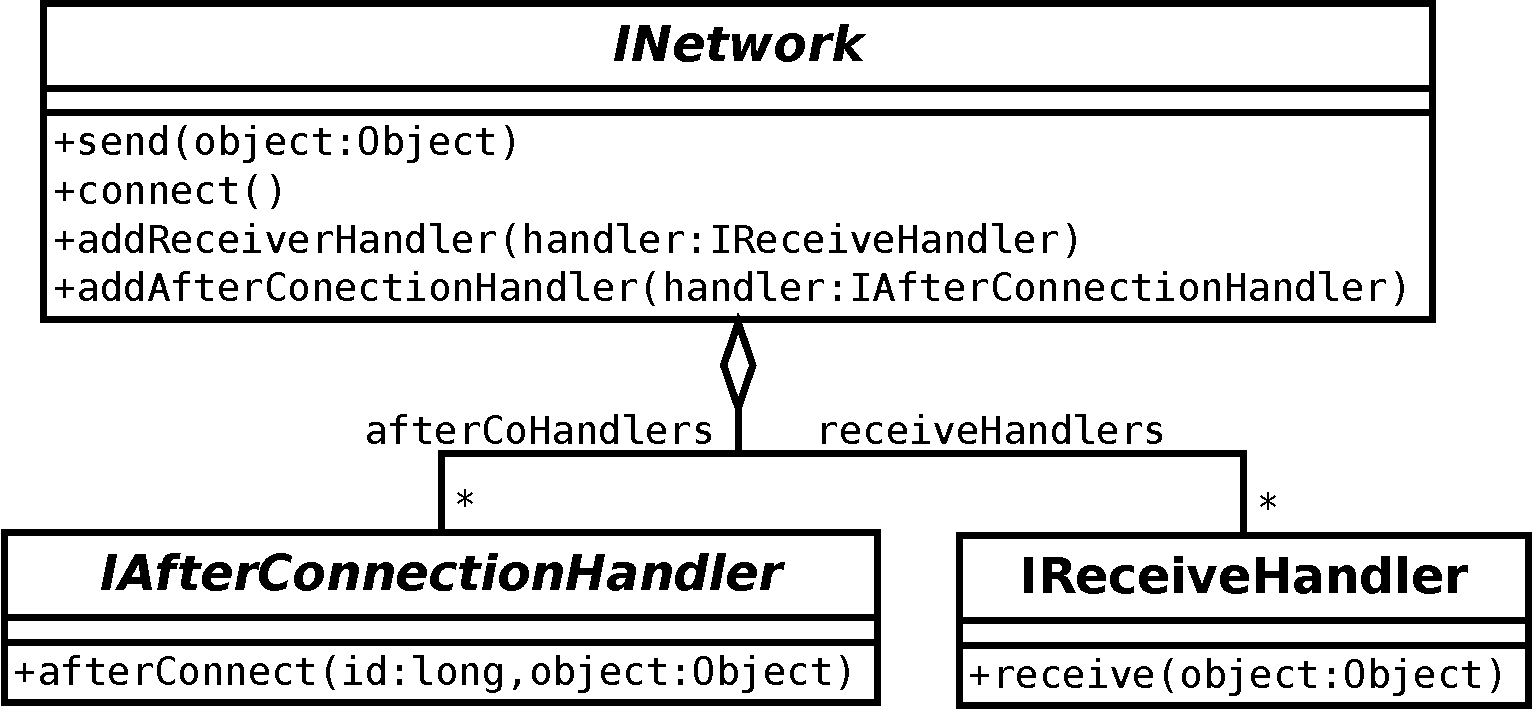
\includegraphics[scale=.3]{includes/model/INetwork.pdf}
    \end{figure}
    \begin{itemize}
      \item Envoi et Réception de messages.
      \item Callback après la connexion.
      \item Callback après la réception de messages.
    \end{itemize}
  \end{frame}

  \begin{frame}
    \frametitle{UI}
    \begin{figure}
    \center
		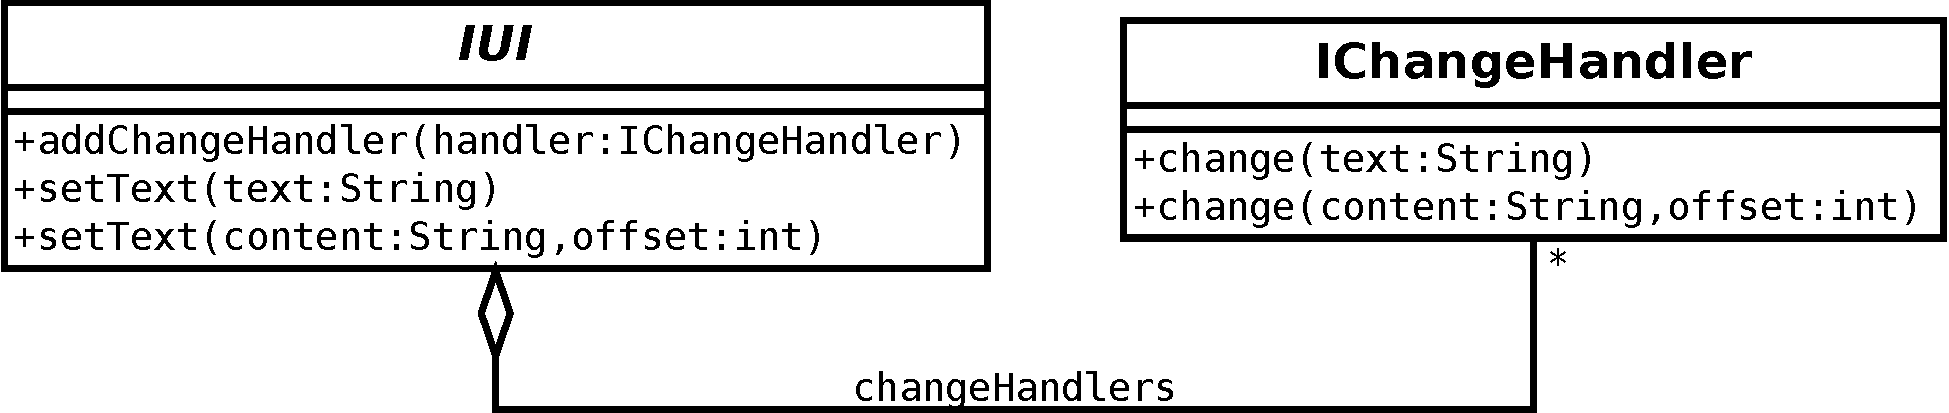
\includegraphics[scale=.3]{includes/model/IUI.pdf}
    \end{figure}
    \begin{itemize}
      \item Visionner et modifier le document texte.
      \item Callback à la modification du texte.
    \end{itemize}
  \end{frame}

  \begin{frame}
    \frametitle{Controller}
    \begin{figure}
    \center
		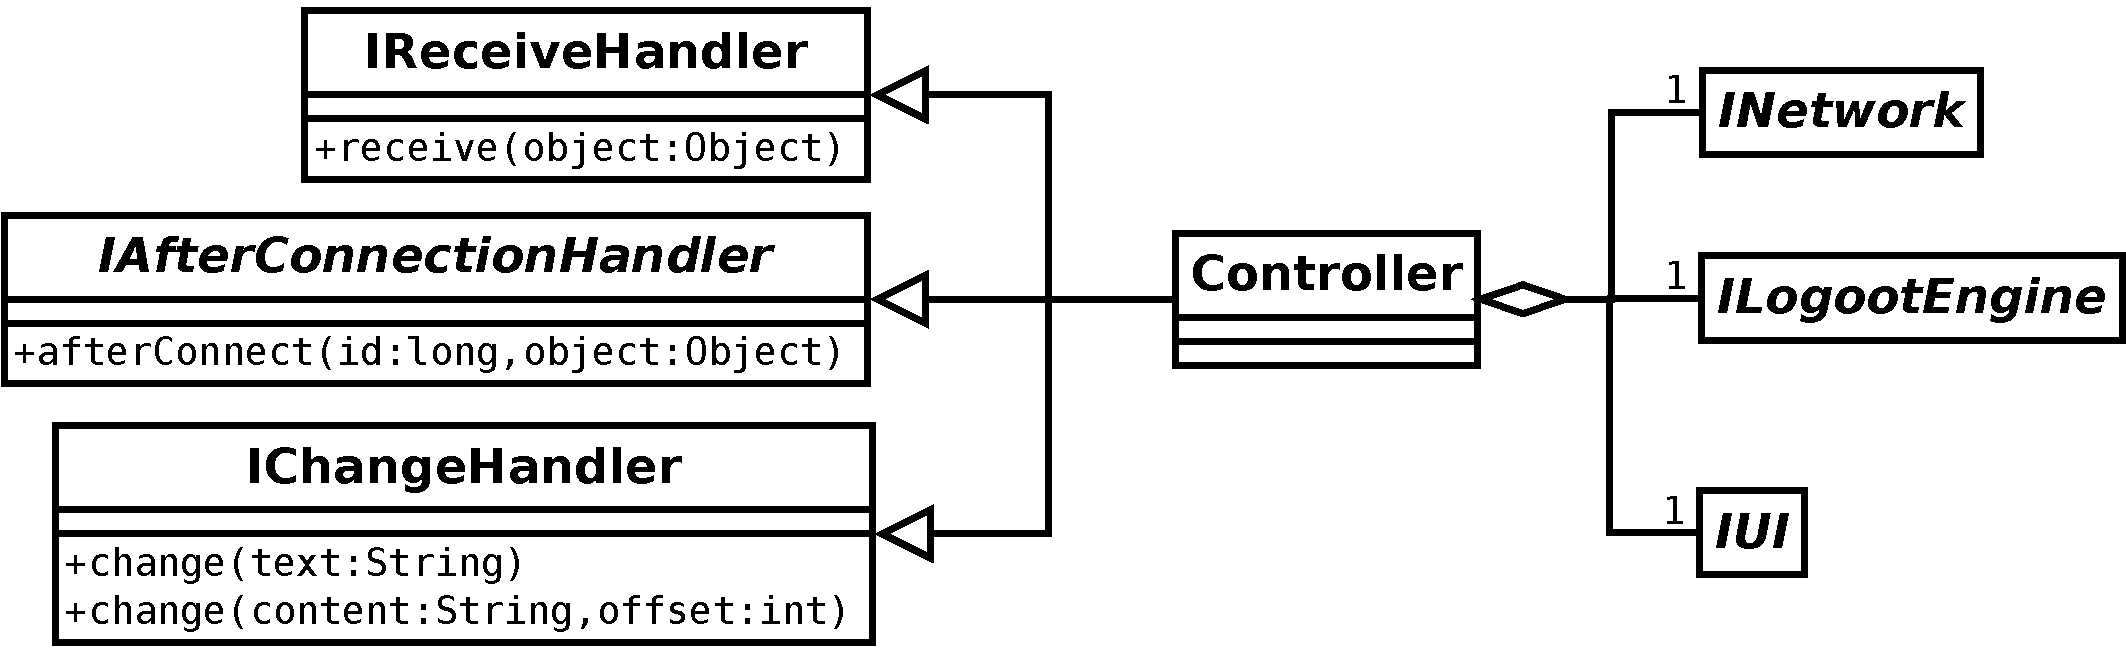
\includegraphics[scale=.3]{includes/model/Controller.pdf}
    \end{figure}
    \begin{itemize}
      \item Lie les composants.
      \item Implémente les callbacks.
    \end{itemize}
  \end{frame}

